\section{Ponteiros}

\begin{frame}[fragile]{Definição de ponteiros}
	\begin{itemize}
		\item Um {ponteiro} é uma variável que contém um {endereço de memória}, normalmente a 
        posição de {outra variável} na memória

		\item Se uma variável contém o endereço de {outra}, então diz-se que a primeira variável 
        {aponta} para a segunda
	\end{itemize}

    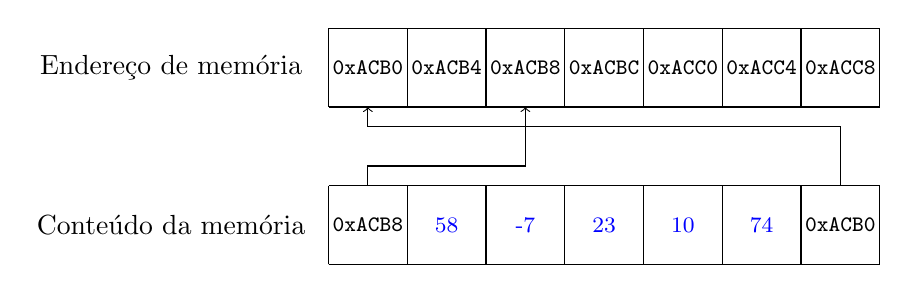
\begin{tikzpicture}
        \node at (0, 2.5) {Endereço de memória};
        \draw (2,2) grid (9,3);
        \node at (2.5,2.5) {\footnotesize \texttt{0xACB0}};
        \node at (3.5,2.5) {\footnotesize \texttt{0xACB4}};
        \node at (4.5,2.5) {\footnotesize \texttt{0xACB8}};
        \node at (5.5,2.5) {\footnotesize \texttt{0xACBC}};
        \node at (6.5,2.5) {\footnotesize \texttt{0xACC0}};
        \node at (7.5,2.5) {\footnotesize \texttt{0xACC4}};
        \node at (8.5,2.5) {\footnotesize \texttt{0xACC8}};

        \node at (0, 0.5) {Conteúdo da memória};
        \draw (2,0) grid (9,1);
        \node at (2.5,0.5) {\footnotesize \texttt{0xACB8}};
        \node at (3.5,0.5) {\footnotesize \textcolor{blue}{58}};
        \node at (4.5,0.5) {\footnotesize \textcolor{blue}{-7}};
        \node at (5.5,0.5) {\footnotesize \textcolor{blue}{23}};
        \node at (6.5,0.5) {\footnotesize \textcolor{blue}{10}};
        \node at (7.5,0.5) {\footnotesize \textcolor{blue}{74}};
        \node at (8.5,0.5) {\footnotesize \texttt{0xACB0}};

        \draw[->] (2.5,1) -- (2.5,1.25) -- (4.5,1.25) -- (4.5,2);
        \draw[->] (8.5,1) -- (8.5,1.75) -- (2.5,1.75) -- (2.5,2);
    \end{tikzpicture}
\end{frame}

\begin{frame}[fragile]{Sintaxe para ponteiros}

    \metroset{block=fill}
    \begin{block}{Sintaxe para declaração de ponteiros}
        \inputsyntax{c}{ponteiros.st}
    \end{block}

	\begin{itemize}
		\item Observe que a sintaxe é idêntica à de declaração de variáveis, com exceção
        do símbolo \code{c}{*} 

		\item É uma boa prática inicializar um um ponteiro no momento de sua declaração

        \item O valor 0 (zero) não é um endereço válido, e indica um ponteiro nulo

		\item Existem dois operadores unários associados à ponteiros:

        \begin{enumerate}
		\item O operador \code{c}{&} (endereço de) devolve a posição que seu operando 
        ocupa na memória

		\item O operador \code{c}{*} (valor de), quando aplicado a um ponteiro, retorna o 
        valor armazenado no endereço de memória apontado
        \end{enumerate}
	\end{itemize}

\end{frame} 

\begin{frame}[fragile]{Exemplo de uso de ponteiros}
    \inputcode{c}{ponteiros.c}
\end{frame}

\begin{frame}[fragile]{Aritmética de ponteiros}

	\begin{itemize}
		\item As únicas duas operações aritméticas que podem ser feitas entre ponteiros e inteiros 
        são a adição e a subtração

		\item Porém o valor indicado não é somado diretamente ao endereço: na verdade o ponteiro 
        se movimenta o número de posições indicadas pelo inteiro, de acordo com o 
		tamanho do tipo de dado do ponteiro
		
		\item A subtração funciona de forma similar à adição

		\item Os ponteiros podem ser incrementados ou decrementados, ou podem estar envolvidos em 
        expressões que envolvam somas e subtrações entre um ponteiro e uma variável inteira

		\item Ao ser incrementado, o endereço apontado pelo ponteiro não é acrescido em uma 
        unidade: o ponteiro é deslocado para o próximo elemento do tipo de dado do ponteiro
	\end{itemize}

\end{frame}

\begin{frame}

	\frametitle{Aritmética de ponteiros}

	\begin{itemize} 
        \item Ao contrário das variáveis, é possível declarar ponteiros do tipo 
        \code{c}{void}

        \item Ponteiros para o tipo \code{c}{void} armazenam endereços de memória de
        tipo não especificado, de modo que não é possível utilizar o operador 
        \code{c}{*} em tais ponteiros

		\item Também não é possível realizar aritmética de ponteiros 
		com um ponteiro do tipo \code{c}{void}

		\item A diferença entre dois ponteiros do mesmo tipo 
		resulta em um inteiro que indica o número de elementos
		daquele tipo entre os dois ponteiros

		\item A soma de dois ponteiros não tem sentido prático e não é permitida
	\end{itemize}

\end{frame}

\begin{frame}[fragile]{Exemplo de aritmética de ponteiros}
    \inputcode{c}{aritmetica_de_ponteiros.c}
\end{frame}

\begin{frame}[fragile]{Vantagens e desvantagens do uso de ponteiros}

    \begin{tabular}{p{5cm}p{5cm}}
    \toprule
    \textbf{Vantagens} & \textbf{Desvantagens} \\
    \midrule
    O uso de ponteiros permite a uma função modificar o valor de seus argumentos &
    Ponteiros não inicializados podem causar uma pane no sistema \\
    \midrule
    \rowcolor[gray]{0.9}
    Os ponteiros são utilizados para dar suporte às rotinas de alocação dinâmica de memória &
    Erros no uso de ponteiros são fáceis de cometer e difíceis de se encontrar \\
    \midrule
    O uso de ponteiros pode aumentar a eficiência computacional de algumas rotinas &
	A gerência da memória fica a cargo do programador \\
    \bottomrule
    \end{tabular}
\end{frame}   
